\documentclass[a4paper]{article}

\usepackage{amsmath}
\usepackage{amsfonts}
\usepackage{amssymb}
\usepackage{url}
\usepackage{graphicx}

\title{Kinect Virtual Dressing Room}

\author{Fedde Burgers \\ 5705509 \\ \texttt{f.j.b.burgers@uva.nl} \and Morris Franken \\ 6151825 \\ \texttt{morrisef@science.uva.nl} \and Carsten van Weelden \\ 0518824 \\ \texttt{cweelden@science.uva.nl}}

\begin{document}

\maketitle

\begin{abstract}

\end{abstract}

\par\noindent {\small{\em Keywords\/}: augmented reality, virtual clothing, user tracking, kinect}

\section{Introduction}
\label{sec:introduction}

The gaming industry has recently introduced the Kinect sensor which has interesting academic applications. It allows one to generate a depth image alongside a RGB camera image and comes with tools that provide human pose detection and tracking. These abilities are used by the gaming industry to allow users to control games using body movement. It can also be used to create an immersive virtual reality presence for the user such as in the Kinect Superman project\footnote{\url{https://github.com/kinectsuperman/Kinect-Superman}} and also to create augmented reality applications in which virtual objects seem to interact with the user and his environment.

In this project we use the Kinect sensor to create an augmented reality dressing room in which the user can try on virtual clothes. The pose of the user is tracked to allow the clothing to move with the user and the depth image is used to create an avatar of the user that approximates the user's body shape. Next, cloth simulation is applied to the virtual clothing to make it move and fold realistically based on the user's movements. The depth image from the sensor is used to compute the girth of the user's body at several places, which can be used to adapt the user avatar, adapt the clothing to the user's body shape, and recommend clothing sizes to the user. The RGB image is used as a background over which the clothing is projected and is displayed on the user avatar when it occludes parts of the clothing. The user is segmented from the background and the intensity of this part of the image is calculated to adapt the lighting of the virtual clothes. This makes the clothing appear as if it is in the same room as the user by reacting to bright and shaded parts of the environment.

\subsection{Project goals}
\label{sec:project_goals}

The focus of this project is to create as realistic an augmented reality dressing room as possible. To accomplish this requires real-time, accurate, tracking of the user pose as well as realistic virtual clothing. For the pose tracking the Kinect sensor is used which gives more complete and accurate tracking of the user pose than the marker based or image-feature based tracking which is traditionally used in augmented reality applications. For the clothing we created a set of 3d models that can be rendered into the scene. The goal of this project is for the user to be able to realistically interact with these virtual pieces of clothing. To achieve this the clothing needs to:
\begin{itemize}
\item be aligned correctly with the user position and pose.
\item move and fold realistically. 
\item be realistically rendered into the environment.
\end{itemize}

The rest of this paper is organized as follows. Section \ref{sec:related_work} discusses previous implementations of the virtual dressing-room concept and organizes them relative to the goals mentioned above. Section \ref{sec:implementation} presents our own implementation and the choices that we made and section \ref{sec:discussion} discusses some of the limitations of our approach. Our conclusions are presented in section \ref{sec:conclussion}.


\section{Related work}
\label{sec:related_work}

Evolution of the virtual dressing room idea: avatar with static clothes, AR with markers, full body with static clothes etc. Dimensions along which to organize: user tracking ability (none, markers, full skeleton tracking), clothing simulation (2d images, static clothes from multiple angles, movable clothes, full physics simulation),

\section{Implementation}
\label{sec:implementation}

\subsection{User tracking}
\label{sec:user_tracking}

\subsection{Virtual clothes}
\label{sec:virtual_clothes}
#clothing, lightness
...
To create of more realistic scene we measure the light conditions of the RGB image. This is done by converting the image to an HSV image and take an average of the intensity from the user.
A point light in Unity will try to recreate the right light conditions.


\subsection{Size estimation}
\label{sec:size_estimation}
On calibrating the user size and length is measured. This information is used to change the user model to fit to the user body. Another feature is to recommend the right size of clothing. The length of each limb is taken by computing the distance between each joint from the skeleton.
The size of the body is taken by estimating the girth of the chest on a number of points.
\begin{figure}[htp]
\centering
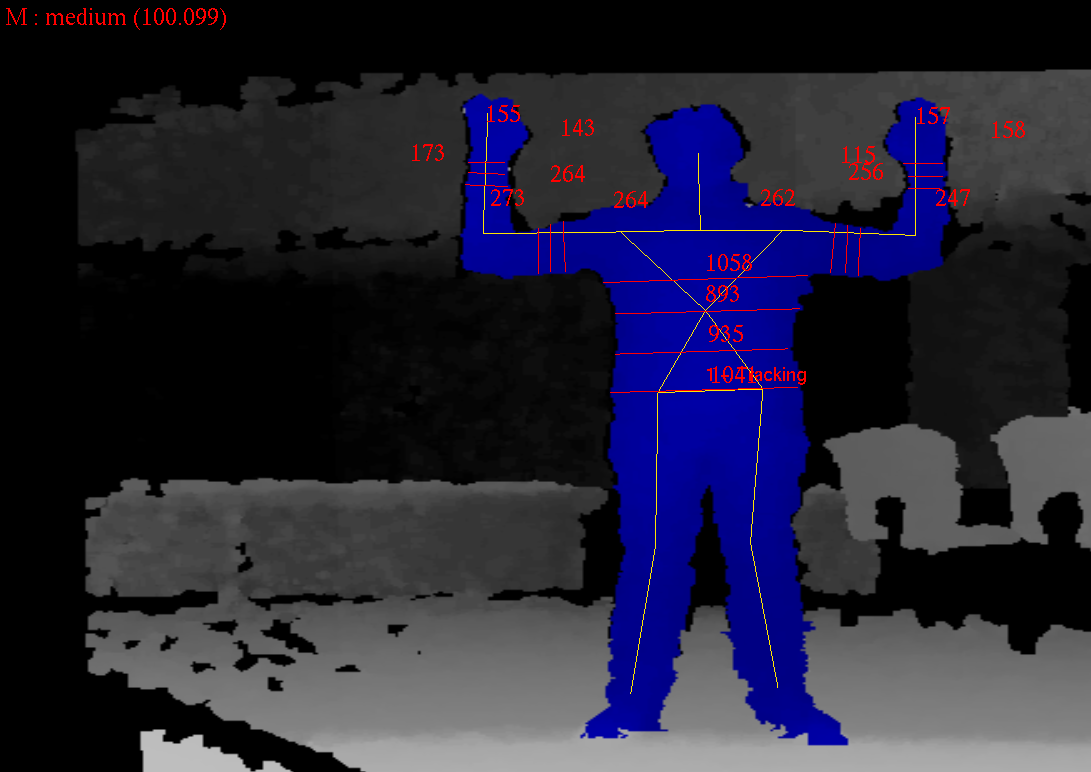
\includegraphics[scale=0.3]{size_estimation.png} 
\caption{size estimation of an user, red lines represent the places where the girth is measured. The numbers are the estimated girth of those lines.}
\label{fig:size_estimation}
\end{figure}
The girth can be measured by two methods:
\begin{itemize}
\item Computing the distance between each point on the line
\item Taking 3 points (outer left, centre and outer right) and compute the distance between those
\end{itemize}
Although the first solution seems the best, it is not robust to a noisy sensor and cloth folding. Even the slightest fold will drastically increase the users estimated girth.
The second option, although no ideal, proved more accurate than the first method.
\\
Because we can only see the front part of the user body, we have to estimate the full girth. This is done by multiplying the front part with a factor 2.1.
Before giving the estimate size of the user, we take the average over 20 frames before drawing an conclusion.

\subsection{Application overview}
\label{sec:application_overview}

Walkthrough, gui, mooie plaatjes

\section{Discussion}
\label{sec:discussion}

Interaction with cloth using collision detection, mislukte interactive cloth approach

Pixel shaders vs user body (zou als groot voordeel hebben dat je ook andere objecten (bv. tafel waar je achter staat) de kleding zouden occlude-en

Evaluatie van size estimation moet grotere dataset hebben

Kleding zou meer realistisch zijn met hulp van 3d artists (textures, pasvorm)

\section{Conclusion}
\label{sec:conclusion}

Evaluation of project goals in section 1
\end{document}